\section{Backend - REST-Schnittstelle und Infrastruktur}
	\subsection{Überblick}
	Das Backend besteht aus mehreren Komponenten. Einerseits muss eine gewisse Software-Infrastruktur aufgebaut werden, um \Gls{webinterface} und die REST-Schnittstelle bereitzustellen. Andererseits muss die Anwendung selbst auch entwickelt werden. Diese besteht wiederum auch aus mehreren Teilen. Darunter fällt die REST-Schnittstelle, inklusive der implementierten Endpoints, selbst, Schnittstellen zu diversen Diensten, wie dem TGM-LDAP Server, zur Datenbank, zu Google Maps und zu WebUntis, aber auch die weitere Funktionalität der Anwendung, unter anderem das Versenden von E-Mails oder Erstellen von PDF-Dateien.
	\\
	\begin{figure}[H]
		\centering
		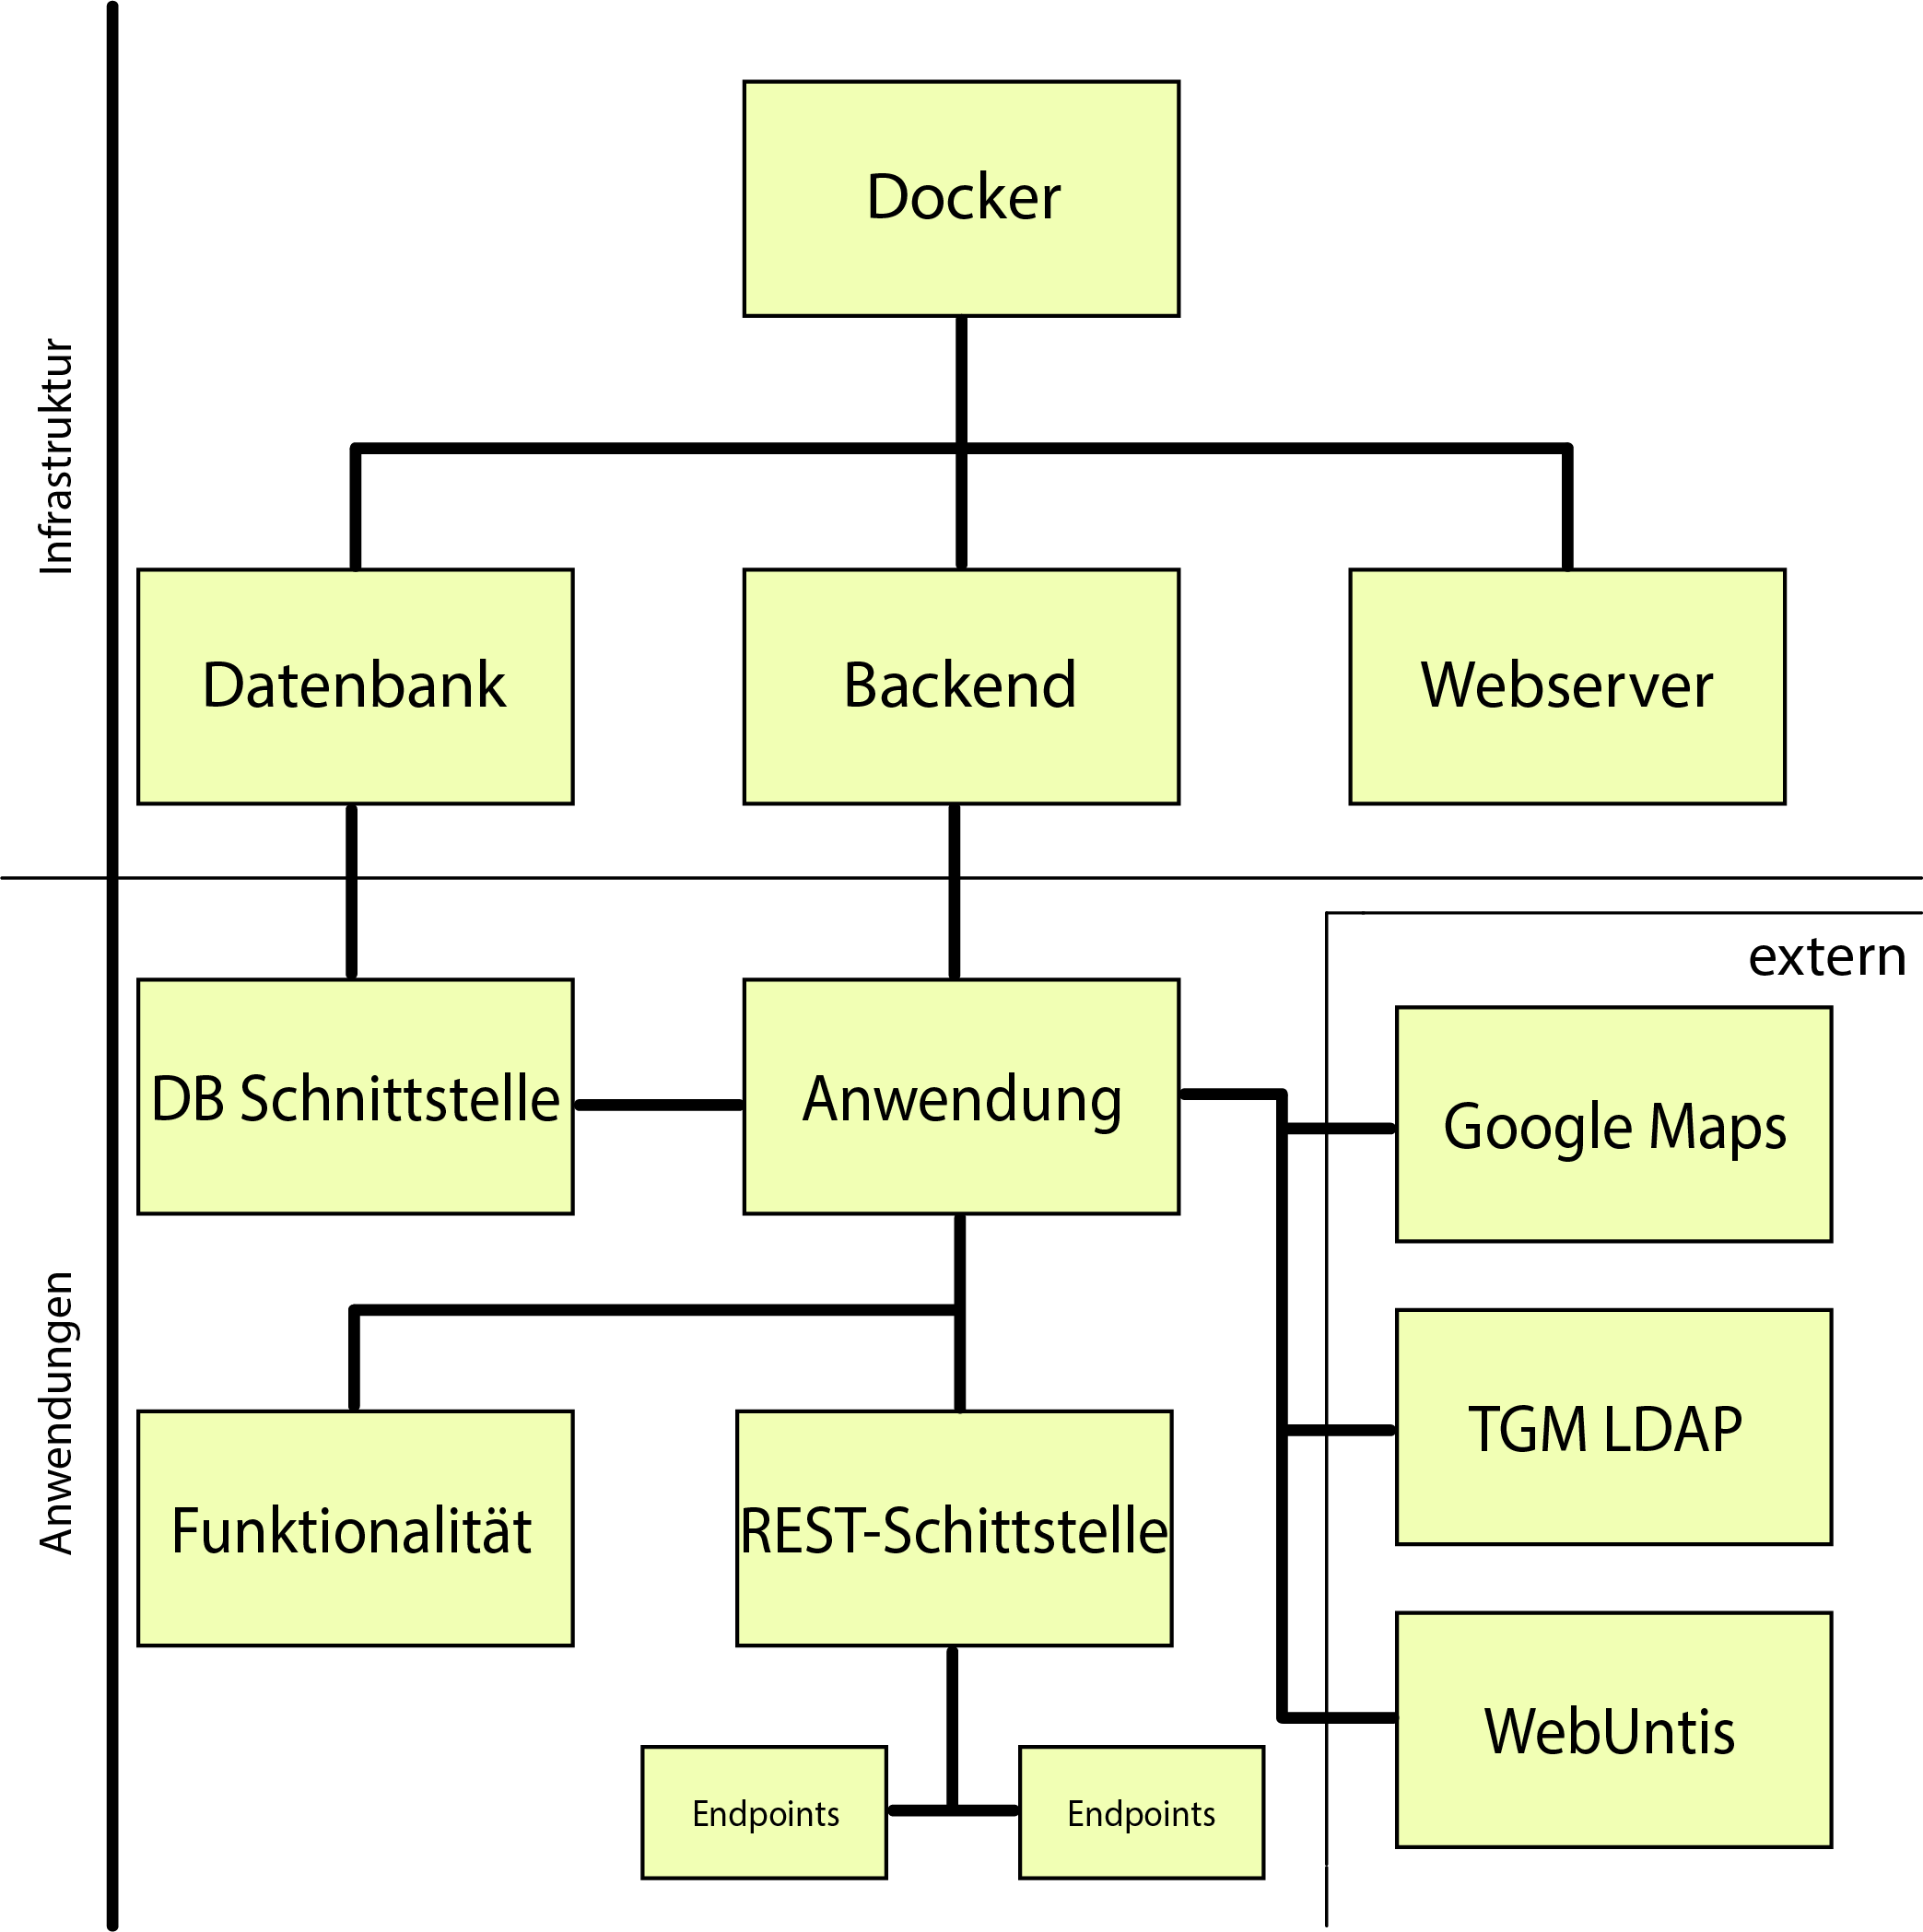
\includegraphics[width=0.8\linewidth]{images/uebersicht}
		\caption[Übersicht über die Komponenten]{Übersicht über die verschiedenen Komponenten der Infrastruktur und der Anwendung}
		\label{fig:uebersicht}
	\end{figure}
	
	\subsection{Docker}
	Um die Infrastruktur des Projektes einfach aufbauen zu können, wird \Gls{docker} genutzt. Da es sich hier um eine komplex strukturierte Infrastruktur handelt wird zusätzlich das Werkzeug \Gls{dcompose} genutzt. Mit Docker Compose kann eine Infrastruktur aufgebaut die der \hyperref[fig:uebersicht]{Abbildung - Übersicht} entspricht. Für diese sind folgende Container vorgesehen, die in den nächsten Kapiteln noch ins Detail beschrieben werden.
		\subsubsection{Datenbank}
		Um die Daten, die durch Refundable erhoben und generiert werden, zu speichern, benötigen wir eine \gls{db}. Auf Grund der Daten, welche sich durch unterschiedliche Datenstrukturen auszeichnen, ist der Einsatz einer \gls{relDb} nicht sinnvoll. Stattdessen empfiehlt sich die Verwendung einer \gls{nosqlDb}.
		
		Standardmäßig wird zwischen 4 verschiedenen Typen von NoSQL Datenbanken unterschieden, welche jeweils nur in ihrem eigenen Use Cases sinnvoll anwendbar sind:
		\begin{itemize}
			
			\item Key-Value Datenbank
			\item spaltenorientierte Datenbank
			\item graphenorientierte Datenbank
			\item dokumentenorientierte Datenbank
		\end{itemize}			
		Bei Key-Value Datenbanken wird einem Schlüssel ein Wert hinterlegt. Dieser Wert ist dann jederzeit über den Schlüssel in der Datenbank abrufbar. Für unseren Use Case ist dieses System nicht sinnvoll anzuwenden, da die von uns benutzten Daten hierfür zu komplex im Aufbau sind.~\\
		Bei spaltenorientierten Datenbanken werden Daten vorrangig über ihre Spalten (statt wie bei relationalen \gls{db}s in Zeilen) analysiert. Dies ermöglicht die einfache Umsetzung statistischer Methoden auf Basis der Spalten. Da jedoch wieder eine Tabelle als Grundstruktur vorliegt, ist dieser Typ von Datenbank nicht sinnvoll anwendbar für Refundable.~\\
		Bei graphenorientierten Daten wird vorrangig auf die Beziehung zwischen einzelnen Elementen geschaut. Daten werden hierbei in Knoten gespeichert, welche zu anderen Verbunden werden können. Die primären Elemente sind hierbei die Beziehungen, anstatt der Daten selbst. Da die Daten von Refundable nicht über starke Beziehungen charakterisiert sind, ist auch dieser \gls{db}-Typ nicht sinnvoll zu benutzen.~\\		
		Zuletzt bei dokumentenorientierten Datenbanken unterliegt jeder Datensatz in einem eigenen Dokument, welches in \Gls{json}, \Gls{yaml}, \Gls{xml} oder ähnlichen Datenformaten gespeichert wird. Dadurch ist auch eine jeweils von einander unabhängige Datenstruktur möglich. Auf Grund der Flexibilität bei Datenstrukturen ist eine dokumentenorientierte Datenbank eindeutig sinnvoll zu verwenden.\cite{nosqltypes}~\\
		Als \gls{dbms} kommt bei dieser Auswahl einige Software in Frage. Die am meisten verbreitete Software hier ist MongoDB und CouchDB. Wo MongoDB auf strenge \gls{konsistenz} setzt, setzt CouchDB auf hohe \gls{verfugbarkeit}. Da in unserem Projekt Konsistenz wichtiger ist als Verfügbarkeit wird MongoDB in einem Container als \gls{dbms} verwendet.\cite{mongo}
		
		\subsubsection{Backend-Container}
		
		Ebenfalls wird ein Container, also eine Umgebung, in dem das Backend laufen kann, erstellt. Dieser wird direkt zu den anderen Containern hinzugefügt, damit dieser über ein Docker-Netzwerk mit den anderen Containern kommunizieren kann.~\\
		Um diesen Container zu realisieren wird als Basis ein alpine-Image genutzt. Dieses stellt eine sehr sparsame Linux-Instanz dar, die in einem eigenem Container laufen kann. Um diesen Container noch entsprechend anzupassen, wird ein entsprechendes Docker-Image über ein Dockerfile gebaut.\cite{alpine}
		
		\subsubsection{Webserver}
		
		Als Webserver um das Webinterface aufrufbar und verfügbar zu machen wird ein Apache2 Server genutzt. Dieser Container ruft automatisch das Frontend auf und kopiert es in seine Umgebung. Ebenfalls muss der Container Zugriff auf Zertifikaten bekommen, um einen sicheren Zugriff über \gls{https} gewährleisten zu können.\cite{apache}
				
	\subsection{Deployment}
	Das Deployment soll automatisch geschehen. Um dies einfach zu ermöglichen, werden die oben zuvor beschriebenen Docker-Container, GitHub und ein Skript, welches die Schritte ausführt, genutzt. Das Skript ist hier der Hauptbaustein, welcher den Vorgang startet und steuert. Zusätzlich zum Installationsvorgang, soll das Skript auch die weitere Steuerung der Software, also starten, stoppen, updaten, cleanen und deinstallieren.~\\
	Das Skript liegt in einem eigenem Install-\Gls{repo}, in welchem sonst keine weiteren Dateien liegen. Dadurch kann es einfach gecloned werden und direkt installiert werden; der Rest wird automatisch erledigt.~\\
	Der Installationsvorgang setzt sich aus folgenden Schritten zusammen:
	\begin{enumerate}
		\item Das Skript macht sich selbst verfügbar durch Setzung von environment variables bzw. dem Kopieren in einen Folder, der in der Path-Variable liegt.
		\item Das Docker-, das Backend-, und das Frontend-Repository werden in Unterordner gecloned.
		\item Docker wird - falls benötigt - automatisch installiert und konfiguriert.
		\item Die individuellen Docker-Images werden über Docker Compose gebuilded.
	\end{enumerate}
	Die Start- und Stoppvorgänge müssen dann nur mit Docker Compose interagieren. Beim Updatevorgang werden die Repositories abgeglichen. Falls eine neue Version verfügbar ist, wird diese heruntergeladen. Die Container werden dann dementsprechend neugestartet. Der Cleanvorgang säubert das System von allen nicht mehr benötigten Docker Containern, Images und Networks. Zuletzt macht der Deinstallationsvorgang einfach den Installationsvorgang rückgängig.
	\subsection{REST-Schnittstelle}
	%Was ist eine REST-Schnittstelle
		\subsubsection{Sprache und Framework}
		%Welche Sprache und Frameworks nutze ich
		\subsubsection{Endpoints}
		%Welche Endpoints wird es geben
	\subsection{Funktionalität}
	Das Backend ist jedoch nicht nur eine reine REST-Schnittstelle, die Daten als Webservice zur Verfügung stellt, sondern auch ein Dienst, der gewisse Funktionalität implementiert und mit anderen Diensten über Schnittstellen kommuniziert. Die Hauptkomponenten und -funktionalität wird in den folgenden Unterkapiteln beschrieben.
		\subsubsection{TGM-LDAP Schnittstelle}
		% Wie interagiere ich mit LDAP
		\subsubsection{Datenbank Schnittstelle}
		% Wie interagiere ich mit Mongo DB
		\subsubsection{Google Maps}
		% Wie interagiere ich mit Google Maps
		\subsubsection{WebUntis}
		% Wie interagiere ich mit WebUntis
		\subsubsection{E-Mails}
		% Wie versende ich E-Mails
		\subsubsection{PDF-Dateien}
		% Wie generiere ich PDF-Dateien
	\subsection{Kommunikation und Datenformate}
	% Forschungsfrage